\chapter{検討手法}
\begin{figure}[ht]
    \centering
    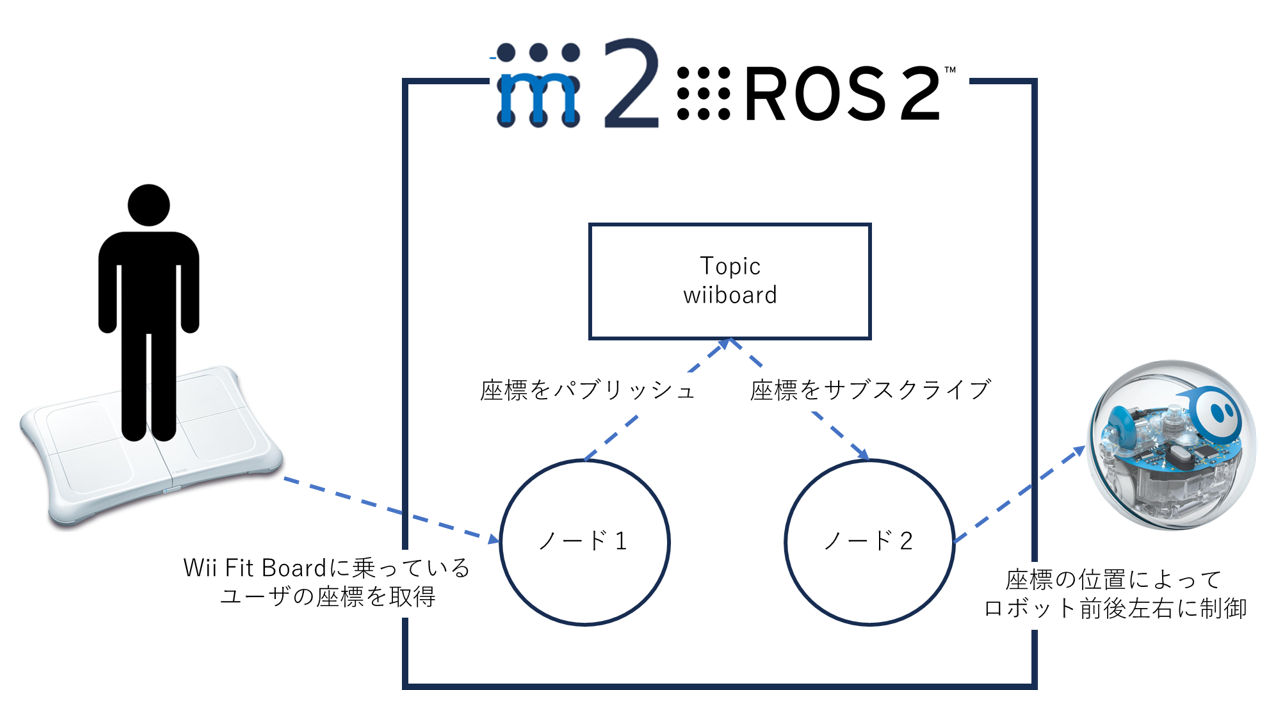
\includegraphics[width=10cm]{images/fig3_application_structure.png}
    \caption{Sphero sprk +とWii Fit Boardを用いたSphero sprk +を制御するアプリケーションの構成図}
    \label{fig:sphero sprk}
\end{figure}
%spheroとraspimouseのwiiboardの手法について話す
%spheroはcgoの話とライブラリ移植の話
%raspimouseは開発環境の話と調査が必要な個所についての話.何と何がうまくいって何がうまくいかなかったのかなど.
この章では,本実装に至らなかったものの検討した手法について述べる.
\section{Sphero sprk+}
Sphero sprk+とWii Fit Boardを用いたロボットの動作を制御するアプリケーションの実装をROS 2とmROS 2-POSIXの2つの環境で行うことを検討した.
図3.1に検討予定だったアプリケーションの構成図を示す.
Sphero sprk +は,Sphero社が発売した球体のロボットで,ユーザーがスマートフォンから操作することができる.
また,Wii Fit Boardは,任天堂が発売したWiiの周辺機器で,体重移動を検知することができる.
この実装を検討し,行った理由は,この実装を行うことで,mROS 2-POSIXとROS 2それぞれの特徴を生かし実験することで,mROS 2-POSIXがユーザーインタラクションにROS 2と違いどのように影響するかを検証することができると考えた.
\\ アプリケーションのノードは2つで主にWiiboardのセンサの値をパブリッシュするノードとその値をサブスクライブしSphero sprk +を制御させるノードで構成されている.
ROS 2側の実装では,Sphero sprk +を動作させるためのライブラリがPythonで提供されていたため,Pythonを用いて実装をおこなった.
ライブラリはSphero sprk +をサーバーに見立てて,マシン側でクライアントコードを書き,サーバーからのレスポンスでSphero sprk +を動作させる仕組みである.
これはbluepyというPythonでBLEデバイスと通信するためのライブラリを用いて実装がされており,Sphero sprk +のライブラリをマシン側でimportすることでimportのライブラリを介してbluepyを使用しSphero sprk +を制御することができた.
そして,このライブラリを用いることで,比較的簡単にSphero sprk +を動作させることができるようになっている.
\\ また,Wii Fit Boardのセンサの値を取得し,Sphero sprk +を制御するノードまでの実装はC++言語で実装を行った.
これはWii Fit Boardの値を取得するプログラムとして参考にしていたプログラムがC++言語で実装されていたため,そのままC++言語で実装をする必要がある.
このプログラムは,Wii Fit Boardを端末とBluetooth接続する必要があり,接続後は/devにある/event○○を開くことでWii Fit Boardのセンサ値を取得できる.
Wii Fit Boardにはセンサが4つあり,接続語の/eventから4つの値が取得できる.
この値をそのままパブリッシュすると,サブスクライブする側で4つの値を処理しなくてはならず,負担が大きいと考え,この4つの値をx,yの2つの値に変換することができた.
座標変換は,Wii Fit Boardのセンサの値をx,yの値に変換するプログラムを参考にして実装を行ったため比較的容易であった.
ROS 2側は先ほど述べたように,スムーズに実装を終えることができた.
\\ しかし,mROS 2-POSIX側では,Sphero sprk +を動作させるためのライブラリがPythonで提供されていたため,PythonをサポートしていないmROS 2-POSIXでは実装を行うことが難しいと考えた.
そこで,bluezというLinux上でBluetoothを扱うためのライブラリを用いて,Sphero sprk +を動作させることを検討した.
bluezを用いることで,Sphero sprk +をBLEサーバーと見立てたクライアントのスクリプトの実装のために,ドキュメントを確認したが,どれも古いものが多く,現在のbluezのバージョンでは動作しないものが多かった.
そのため,bluezを用いてSphero sprk +を動作させることは断念した.
\\ そこで,Sphero sprk +を動作させるライブラリはgo言語にもあったため,cgoと呼ばれるgo言語からC言語の関数を呼び出すための仕組みを用いて,go言語からSphero sprk +を動作させることも試みた.
続けていくと,mROS 2-POSIXのcgo移植になってしまい,実装範囲が広くなってしまったため,実装を断念した.
Wii Fit Boardのセンサの値を取得するプログラムは,C++で実装されていたため,移植は容易だった.
問題は移植後のmROS 2-POSIXで作成したPublisherによるSegment Faultだった.
これはまだ初期化されていない変数や,サブスクリプションのコールバック関数の引数がNULLの場合に発生する.
ビルドを通ることが多いため予測が困難で完全な実装に時間を要した.
このように実装に多くの時間がかかったことが検討で終わってしまった理由の一つではあるが,もう一つの理由として,実験を通して有用性のあるデータの取得が困難だったことが挙げられる.
システム上,一本道であるためRound Tripのような実行速度を比較する実験が難しく,単純に実行時間の比較実験ができなかった.
心理学実験のような実験を行うことで,ユーザーインタラクションにどのような影響があるかを検証することができると考えたが,集められたデータに信頼性を持たせるのが難しいと判断し断念した.
\section{Raspberry Pi Mouse}
Wii Fit BoardとRaspimouseを用いたロボットの動作を制御するアプリケーションの実装を検討した.
Raspimouseとは,ロボット開発キットであるRaspberry Pi Mouseのことで,Raspberry Pi上で動作するROS 2のノードで制御することができる.
Wii Fit Boardは,任天堂が発売したWiiの周辺機器で,体重移動を検知することができる.
このアプリケーションは,Wii Fit BoardからのセンサデータをRaspimouseにPub/Sub通信を用いて送信し,Raspimouseは受信したセンサデータをもとに動作を制御する.
ユーザの体重移動によってロボットが動作するため,ユーザーインタラクションが豊富なアプリケーションを想定した.
このようなユーザーインタラクションが豊富なアプリケーション上で,mROS 2-POSIXとROS 2のアプリケーション上の違いを検証することで,mROS 2-POSIXから新たな知見を得ることができると考えた.
\\ 実装アプリケーションはROS 2とmROS 2-POSIXの2つの環境で動作する.
ROS 2側のアプリケーションは,C++言語でWii Fit Boardのセンサの値をパブリッシュするノードを実装した.
センサの値をパブリッシュするためには,Wii Fit Boardを端末とBluetooth接続する必要がある.
接続後は/devにある/event○○を開くことでWii Fit Boardのセンサ値を取得できる.しかし,/eventはネットワーク環境によってランダムな/event番号に振り分けられるため,実行するネットワーク環境に変更があるたびに修正しなくてはならない.
また,ノード実行前に/dev/uinputにchmodでa+rwの権限を与えておく必要がある.
ネットワークを確認し,パーミッションを確認するとWii Fit Boardの4つのセンサから,センサの値を/eventを通して取得できる.
この値をこのままパブリッシュすると,サブスクライブする側で4つの値を処理しなくてはならないので,この値をx,yの2つの値に変換する.
x,yはユーザの重心点を表しており,Boardに乗っているユーザの体重に応じてその大きさが変化する.
この特性を生かした制御方法でアプリケーションの実装を行った.
\\ 次に,サブスクライブするノードでは,パブリッシュされたx,yの値を受け取り,x,yの値に応じてRaspimouseの動作を制御する処理を実装した.
x,yの値はそれぞれユーザの体重によって大きく増減するため,適切な閾値の値はユーザーによって変化する.
今回の場合は,評価実験するユーザーとして開発者のみになるため,開発者の体重に合わせた閾値の値を設定した.
ロボットが動作する処理は,x,yの値が閾値を超えた場合にRaspimouseが動作するように実装した.
ユーザーがロボットを前進させようとした時,yの値がマイナスに大きく傾くため,yの値がマイナスの閾値を超えた場合にRaspimouseが前進するように実装した.
同様に,yの値がプラスに傾くとき,ロボットを後退させ,xの値がマイナスに傾くときにロボットを右に移動させ,プラスに傾くときにロボットを左に移動させるように実装を行った.
ロボットを移動させる処理はロボットのデバイスドライバを直接write命令を用いてたたくことで実装を行っている.
mROS 2-POSIX側のアプリケーションは,ROS 2側のアプリケーションと大きく変更されていない.
ROS 2側のアプリケーションと同様にWii Fit Boardのセンサの値をパブリッシュするノードを実装し,その値をサブスクライブするノードを実装した.
パブリッシュするノードではROS 2側と同様の実装になっている.
\subsection{実装に際しての課題}
実装に際しての課題としてWii Fit Boardの値をパブリッシュするノードとその値をサブスクライブし,Raspimouseを動作させるノードそれぞれであった.
Wii Fit Boardの値をパブリッシュするノードでは,mROS 2-POSIX側のノードで実行後にSegment Faultが発生した.
mROS 2-POSIXを利用していると,ビルドが成功し,実行時にパブリッシャーとサブスクライブの通信準備が完了した後,Segment Faultが発生することがある.
これによって,ノードが突然動作しなくなる問題があったが,プログラムを書き直し,不正なアクセスが変数にされていないか確認しデバックすることで解決した.
\\ Wii Fit Boardのセンサの値をサブスクライブするノードでは,Raspimouseを動作させる部分で課題があった.
Raspimouseを制御する方法としてROS 2を利用する方法が一般的である.Raspimouseは公式にROS 2ディストリビューション向けにソースビルドのドキュメントやバイナリをaptで配布しており,
そうしたものを手軽にインストールしros2 run, launchで立ち上げることで制御することができた.
また,すでにキーボードやゲームコントローラを使ってRaspimouseを操作できるノードも配布されている.
こうした状況下であったためROS 2側では,比較的容易に動作させることができた.
しかし,mROS 2-POSIX側でRaspimouseの制御ノードのRトピックに対してパブリッシュを動作させると,トピックに値が送信されていないようだった.
デバックツールとしてros2 topic list, info, echo, pubを用いて確認したところ,topic listにmROS 2-POSIXのトピック名を確認できたが,echoによってトピックをのぞくと何も値がpublishされていないようだった.
\\ 原因は,制御ノードがパブリッシュしている値のQoS設定がRELIALBEになっていたためである.
mROS 2-POSIXでは,QoS設定のうち,RELIABLEとBEST\_EFFORTの2つの設定が可能である.
mROS 2-POSIXのQoS設定を変更し,ノードを立ち上げると通信できるはずだが,PCとラズパイマウス間での通信は望めなかった.
問題はQoSではなく,mROS 2-POSIXのノードがパブリッシュしている値をサブスクライブするノードが受け取れていないことにあった.
原因は不明であるが,デバックツールを使っても,mROS 2-POSIX側で値が受け取ることができることなく,ROS 2同士では問題鳴く通信できた.
また,Sphero sprk +と同様に実験で得られるデータの有用性の低さが課題であった.
Sphero sprk +と同様に,システム上,一本道であるためRound Tripのような実行速度を比較する実験が難しく,単純に実行時間の比較実験ができなかった.
そのため,実装を断念した.